\documentclass[12pt,twoside,a4paper]{article}
\usepackage{graphicx}  % Let graphics files be included using \includegraphcs
\usepackage{hyperref}  % Generate hypertext links in references, the index etc.
\usepackage{bm}        % Provides the \bm{x} command for typesetting bold math.
\usepackage{amsmath}
\usepackage{amssymb}
\usepackage{natbib}

\newcommand{\sha}{\mbox{\small I\!I\!I}}
\newcommand{\arcsec}{''}
\newcommand{\nm}{\mbox{nm}}

\newcommand{\ft}{\mathcal{F}}
\newcommand{\ift}{\mathcal{F}^{-1}}
\newcommand{\ftarrow}{\stackrel{\mbox{\scriptsize\it FT}}{\rightarrow}}

\newcommand{\sky}{\mathbf{s}}
\newcommand{\psf}{\mathbf{p}}
\newcommand{\img}{\mathbf{f}}
\newcommand{\msky}{\mathbf{s_m}}
\newcommand{\hsky}{\mathbf{s_h}}
\newcommand{\mpsf}{\mathbf{p_m}}
\newcommand{\hpsf}{\mathbf{p_h}}
\newcommand{\mepsf}{\mathbf{p'_m}}
\newcommand{\hepsf}{\mathbf{p'_h}}
\newcommand{\Mepsf}{\mathbf{P'_m}}
\newcommand{\Hepsf}{\mathbf{P'_h}}
\newcommand{\hlpf}{\mathbf{a_h}}
\newcommand{\Hlpf}{\mathbf{A_h}}
\newcommand{\mimg}{\mathbf{f_m}}
\newcommand{\himg}{\mathbf{f_h}}
\newcommand{\Mimg}{\mathbf{F_m}}
\newcommand{\Himg}{\mathbf{F_h}}
\newcommand{\msha}{\mathbf{\sha_m}}
\newcommand{\hsha}{\mathbf{\sha_h}}
\newcommand{\mnoise}{\mathbf{n_m}}
\newcommand{\hnoise}{\mathbf{n_h}}
\newcommand{\mrawnoise}{\mathbf{\eta_m}}
\newcommand{\hrawnoise}{\mathbf{\eta_h}}
\newcommand{\mdx}{\bm{\delta}_{\dx}}
\newcommand{\mdy}{\bm{\delta}_{\dy}}
\newcommand{\Mdxy}{e^{-2\pi i(\bm{\nu_x}.\varepsilon_x + \bm{\nu_y}.\varepsilon_y)}}
\newcommand{\dx}{\varepsilon_x}
\newcommand{\dy}{\varepsilon_y}
\newcommand{\wt}{\bm{w}}
\newcommand{\Wt}{\bm{W}}

\newcommand{\mgain}{g_m}
\newcommand{\hgain}{g_h}
\newcommand{\gain}{g_v}
\newcommand{\mbg}{b_m}
\newcommand{\hbg}{b_h}
\newcommand{\bg}{b_v}

% Optimize the page layout.

\topmargin 0.0in \headsep 0.0in
\oddsidemargin 0.0in \evensidemargin 0.0in
\textwidth 6.5in \textheight 9.7in
\parindent 0pt
\parskip 12pt

\begin{document}

\vspace{1in}
\begin{center}
{\LARGE\sf Estimating the Point Spread Function of the MUSE Integral
  Field Spectrometer}
\end{center}

\hrule

{\small\bf Martin Shepherd,  $6^{\mbox{th}}$ June 2016}\\

\section{Introduction}

The point-spread function (PSF) of ground-based optical telescopes is
largely determined by atmospheric conditions. Since these conditions
change rapidly, the PSF of each observation is unpredictable.  However
knowledge of the PSF can be important. For example, the shape of the
PSF can be used as a matched filter for detecting faint sources. The
relative PSF widths of multiple observations can also be used to
weight a sum of exposures to optimize the resolution of the summed
image.

The PSF of an image can be estimated directly if the image contains
any isolated stars. The appearance of each star is essentially an
image of the PSF, scaled by the flux of the star. The PSF is harder to
estimate when the image only contains resolved sources or weak point
sources. This document describes one way to estimate the PSF in such
cases, by comparing the ground based images to higher resolution
images from the Hubble Space Telescope (HST). This technique is
primarily designed for observations with Integral Field Spectrometers
(IFS), provided that their wavelength coverage encompasses the
bandpasses of one or more HST imaging filters. In particular, it was
developed for use with the \textit{Multi Unit Spectroscopic Explorer}
(MUSE) on the Very Large Telescope (VLT) in Chile.  It can be used to
determine the relative PSF widths of individual exposures, so that
they can be weighted appropriately when they are combined. More
importantly it can be used to estimate the PSF characteristics of the
final cube of images as a function of wavelength, to facilitate
subsequent photometric analysis.

\section{An Overview of the Procedure}

\begin{figure}[htbp]
\begin{center}
\begin{minipage}[b]{5.5in}
\begin{center}
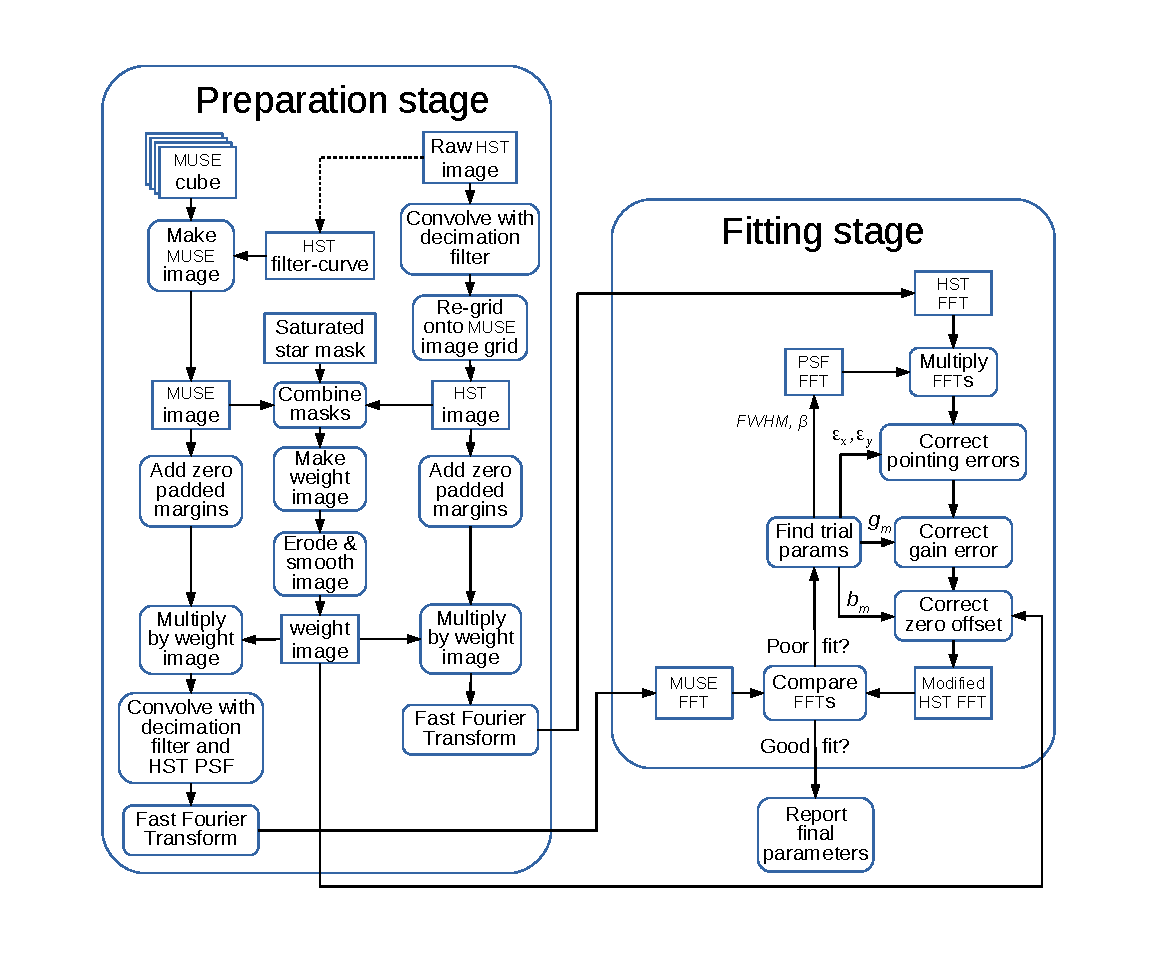
\includegraphics[width=4.5in]{psf_fitting_procedure.pdf}
\caption{An overview of the major steps in the PSF fitting procedure.}
\label{psf_fitting_procedure_figure}
\end{center}
\end{minipage}
\end{center}
\end{figure}

Figure~\ref{psf_fitting_procedure_figure} provides a high-level
overview of the main steps of the PSF fitting procedure. Subsequent
sections describe the underlying reasons for these steps, and how they
are performed.

The underlying rationale of the procedure is that if one had a perfect
high resolution image of the sky, then one could determine the PSF of
a real low-resolution image by convolving the perfect image by a
succession of guesses at the PSF, until a good match to the real image
was obtained. In practice, in place of a perfect image of the sky, an
HST image is used that covers the same region as the target image. In
this document, the image whose PSF is to be determined, will be a MUSE
image derived from a cube of narrow-band images.

In figure~\ref{psf_fitting_procedure_figure}, the procedure is shown
divided into two stages. In the \textit{Preparatory Stage}, the known
properties of a target MUSE image and a corresponding HST image are
used to modify these images until the only differences between them
should be the effect of the MUSE PSF on the MUSE image. These steps
decimate and re-grid the HST image onto the coordinate grid of the
MUSE image, apply the same decimation filter and the HST PSF to the
MUSE image, then arrange that any missing areas in either image are
masked in both images. They also smoothly taper down the edges of the
image and the edges of masked regions, to reduce the effects of
pointing errors on the PSF fitting procedure.

The steps of the subsequent \textit{Fitting Stage} then attempt to fit
for the PSF of the MUSE image by convolving the modified HST image by
a sequence of guesses at the MUSE PSF, until the difference between
the two images is minimized. Simultaneously, the minimizing algorithm
also solves for telescope pointing errors and flux calibration
errors. These steps are performed in the Fourier plane. This is
because PSF convolution and position corrections are much more
efficient in the Fourier plane than in the image plane.

\section{Initial Development for Perfect Telescopes}

The foundations of the technique will be introduced in this
section. They will be described initially as though the MUSE and HST
observations were from perfect telescopes that didn't have gain
errors, pointing errors, noise or background subtraction
errors. Subsequent sections will adjust the technique to take account
of these issues.

For the MUSE observation whose PSF is to be measured, let the flux
distribution on the sky be, $\msky$, the point-spread function of the
observation be, $\mpsf$, and the discrete sampling of the image, be
the Dirac comb, $\msha$. In terms of these functions, the MUSE image
of the sky can be written as follows. Note that $\ast$ denotes
convolution, and $\cdot$ indicates multiplication.

\begin{equation}
\mimg = \msha\cdot (\mpsf \ast \msky)
\end{equation}

The multiplication by the sampling function, $\msha$, on the right
hand side of this equation, means that $\mimg$ only has values at each
delta function of $\msha$, so this equation can equally be written as
follows.

\begin{equation}
\label{muse_image_eqn}
\msha \cdot \mimg = \msha\cdot (\mpsf \ast \msky) \hspace{1in} \mbox{[MUSE]}
\end{equation}

The HST observation that provides the reference image will generally
have a different pointing center, a different orientation on the sky,
and be sampled on a finer grid. The HST image should thus be rotated
to the orientation of the MUSE image, then resampled and cropped, such
that its pixels sample the same positions on the sky as the MUSE
image. If this re-gridded HST image is denoted, $\himg$, then its view
of the sky is as follows.

\begin{equation}
\label{hst_image_eqn}
\msha \cdot \himg = \msha \cdot (\hlpf \ast \hpsf \ast \msky) \hspace{1in} \mbox{[HST]}
\end{equation}

This samples the same patch of sky, $\msky$, as the MUSE image, and
has the same sampling grid, $\msha$. However the PSF, $\hpsf$, of the
original HST image has been convolved with a new term called,
$a_m$. This term represents the low-pass decimation filter that has to
be applied before subsampling the $0.03\arcsec$ samples of the HST
image to the $0.2\arcsec$ samples of the MUSE image. Without this
filter, high spatial frequencies in the HST image would be aliased to
lower spatial frequencies, producing artifacts and noise. More
importantly, the discrete convolutions that are fundamental to the PSF
measuring technique would be invalidated, as described in
section~\ref{discrete_convolution}.

In appendix~\ref{sampling_appendix}, it is shown that for any
continuous functions, $b$ and $c$, $(\sha \cdot b)\ast (\sha \cdot
c)$ is equivalent to $b \ast c$, provided that both $b$ and $c$ do not
contain any frequency components above half the sampling rate of the
sampling function, $\sha$. For this reason, the sampling functions
will be omitted from subsequent equations. 

Appendix~\ref{sampling_appendix} also shows that convolution is both
commutative and associative, so a sequence of convolutions in an
equation like $b \ast c \ast d$ can be performed in any order. With
this knowledge, the right hand sides of equations~\ref{muse_image_eqn}
and \ref{hst_image_eqn} could be made identical by first convolving
the MUSE image with the decimation-filter and the PSF of the HST
image, and then by convolving the HST image with the PSF of the MUSE
image. However since the precise PSFs of the two telescopes are
unknown, estimates are used instead. If $\hepsf$ is the estimated HST
PSF, and $\mepsf$ is the estimated MUSE PSF, then this procedure
results in the following equations.

\begin{eqnarray}
\label{ideal_muse_conv}
\mimg \ast \hlpf \ast \hepsf &=& \hlpf \ast \hepsf \ast \mpsf \ast \msky
\hspace{1in} \mbox{[MUSE]}\\
\label{ideal_hst_conv}
\himg \ast \mepsf &=& \hlpf \ast \hpsf \ast \mepsf \ast \msky
\hspace{1in} \mbox{[HST]}
\end{eqnarray}

The convolutions on the right-hand side of the two equations have
been deliberately reordered to emphasize the similarities between
these equations. This is allowed because of the commutative property
of convolution.

If the estimates of the PSFs are accurate then the images calculated
on the left hand sides of the above two equations should be identical,
so this provides a way to check whether a particular guess at the MUSE
PSF is correct.  Unfortunately, the images will also match if an error
in the estimate of $\hepsf$ is countered by a similar error in the
estimate of $\mepsf$. However if a reasonable estimate of $\hepsf$ can
be determined in advance, then successive guesses at the MUSE PSF,
$\mepsf$, can be tested by a least-squares comparison of the two
images. This is the basis of the technique for finding the PSF of a
MUSE image. A reasonable model of the HST PSF is found. Then the MUSE
PSF is modeled as a Moffat function, and its two free parameters are
varied until the difference between the processed MUSE and HST images
is minimized in a least-squares sense.

The PSF of the HST is much narrower than the MUSE PSF, so a fractional
error in the estimated size of the HST PSF results in a much smaller
fractional error in the fitted size of the MUSE PSF. This means that
the model of the HST PSF does not need to be very accurate to yield a
reasonable estimate of the MUSE PSF. In practice, a circularly
symmetric Moffat model of the HST PSF is used. The free parameters of
are found by model-fitting to a star, using an HST image that was
observed in the same way as the HST image that is used for fitting the
MUSE PSF.

\section{Accounting for flux and position calibration errors}

The equations of the previous section did not take account of pointing
errors, background subtraction offsets, or gain errors. This section
extends the basic technique to cope with these issues. In later
sections, the technique will be further extended to handle unsampled
regions of the sky, image saturation, and geometric distortions.

The MUSE and HST images each have different gain errors, background
subtraction offsets and pointing offsets. However for the purpose of
fitting the PSF of the MUSE image, only the relative errors are
needed. If the flux scale, flux offset and the x-axis and y-axis
pointing errors of the MUSE image, relative to the HST image are
represented by $\mgain$, $\mbg$, $\dx$ and $\dy$, respectively, then
to account for these, equations~\ref{ideal_muse_conv} and
\ref{ideal_hst_conv} become as follows.

\begin{eqnarray}
\label{muse_cal_eqn}
\mimg \ast \hlpf \ast \hepsf &=& \mgain
\cdot \hlpf \ast \hepsf \ast \mpsf \ast \msky \ast \mdx \ast \mdy +
\mbg+\mnoise\\
\label{hst_ref_eqn}
\himg \ast \mepsf &=& \hlpf \ast \hpsf \ast \mepsf \ast \msky + \hnoise
\end{eqnarray}

In these equations $\mnoise$ and $\hnoise$ represent random background
noise in the MUSE and HST images, respectively, and $\mdx$ stands for
$\delta(x-\dx)$, which is a delta function at a distance $\dx$ along
the X-axis of the images. The convolution $\msky\ast\mdx$, shifts
$\msky$ a distance $\dx$ along the X-axis, and
$\msky\ast\mdx\ast\mdy$ moves it by $\dx$ and $\dy$ along the X and Y
axes, respectively.

At this point the right hand sides of equations~\ref{muse_cal_eqn} and
\ref{hst_ref_eqn} are clearly not equivalent. To make them equivalent
within the noise, involves convolving the left hand side of
equation~\ref{hst_ref_eqn} with the same position shifting delta
functions, multiplying the result by the same relative gain error,
then adding the relative flux offset. The result is as follows.

\begin{align}
\label{muse_cal_eqn2}
\mimg \ast \hlpf \ast \hepsf
&= \mgain \cdot \hlpf \ast \hepsf \ast \mpsf \ast \msky \ast \mdx \ast \mdy + \mbg+\mnoise\\
\label{hst_cal_eqn2}
\mgain \himg \ast \mepsf \ast \mdx \ast \mdy + \mbg
&= \mgain \cdot \hlpf \ast \hpsf \ast \mepsf \ast \msky \ast \mdx \ast \mdy + \mbg + \hnoise'
\end{align}

Where the term, $\hnoise'$, which equals
$\mgain\cdot\hnoise\ast\mdx\ast\mdy$, is just a scaled and shifted
version of the original random HST detector noise.

At this point $\mgain$, $\mbg$, $\dx$, $\dy$ and $\mepsf$ are the
unknowns that need to be determined by least squares fitting. The left
hand sides of equations~\ref{muse_cal_eqn2} and \ref{hst_cal_eqn2} are
what are actually calculated for the fitting process, while the right
hand sides of these equations show what the resulting images are
expected to contain. The left hand side of
equation~\ref{muse_cal_eqn2} is calculated once, before the fitting
process starts, whereas the left-hand side of
equation~\ref{hst_cal_eqn2} is repeatedly re-calculated for different
trial versions of the unknown parameters, until the difference between
it and equation~\ref{muse_cal_eqn2} is minimized.

\section{Edges, unsampled regions and saturated sources}

If the edge of the MUSE and HST images cuts through a bright source,
and there is any position error between the two images, then one image
will contain more of the source than the other, resulting in a
difference between the images that can not be resolved by shifting the
images. This can end up dominating the residuals between the processed
images, causing incorrect values to be fitted for the flux offset and
gain parameters, which in turn affect the fitted PSF parameters.  To
reduce this effect, both of the images are multiplied by an image of
weights that smoothly decrease from 1 to zero over a narrow margin
just inside all edges of the image.

The edges that are treated in this way are not just the sides of the
images, but also any areas of the images that are not
sampled. Unsampled areas include areas where the HST image does not
fully overlap with the MUSE image, and areas that have been masked due
to instrumental problems, such as bad pixels. Any pixels that are
saturated due to bright sources should also be masked and treated as
unsampled pixels.

The image of weights is first initialized such that pixels that are
sampled by both telescopes are set to 1, while the remaining pixels
are set to zero. To reduce the effect of the edges in this weighting
image, the borders of the islands of unit valued pixels need to be
tapered slowly to zero. This can't be done by simply smoothing the
array of weights. That would smear non-zero values into the unsampled
regions, which should stay masked. Instead the edges of the islands
are first eroded using a square morphological erosion kernel. Then a
square smoothing kernel of the same size is used to smooth the eroded
edges. Using the same size for the erosion kernel and the smoothing
kernel, ensures that the tapered edges extend right up to the
unsampled areas, but don't encroach into them.

For this procedure to work, the width of the kernels used for erosion
and smoothing should be an odd numbers of pixels. In the version of
this procedure that is used for the MUSE instrument, the default
kernel width is 9 pixels. The rationale for this width will be
explained below.

Ideally the weighting image would be applied to the results of
equations~\ref{muse_cal_eqn2} and \ref{hst_cal_eqn2}, to ensure that
the two processed images were identically weighted. However the
purpose of the weighting image is to replace sharply edges regions of
missing data with zeros, and this has to be done before anything can
be done to these images. The initial MUSE image and the re-gridded HST
image are thus multiplied by the weighting image before any other
operations are performed.

\begin{eqnarray}
  \mimg' &=& \mimg \cdot \wt \\
  \himg' &=& \himg \cdot \wt
\end{eqnarray}

The effect on equations~\ref{muse_cal_eqn2} and \ref{hst_cal_eqn2} are
shown below. Note that on the left hand side of
equation~\ref{hst_cal_eqn2} the estimated background offset, $\mbg$
has also be scaled by the weight image, to make the two equations as
similar as possible.

\begin{align}
\label{muse_cal_eqn3}
&\mimg' \ast \hlpf \ast \hepsf = \mgain \cdot \hlpf \ast \hepsf \ast (\wt\cdot(\msky \ast \mpsf \ast \mdx \ast \mdy)) + \mbg\cdot\wt+\mnoise\cdot\wt\\
\label{hst_cal_eqn3}
&\mgain \cdot \himg' \ast \mepsf \ast \mdx
\ast \mdy + \mbg\cdot\wt = \nonumber \\
& \phantom{\mimg' \ast \hlpf \ast \hepsf ={}} \mgain\cdot(\wt\cdot(\hlpf \ast \hpsf \ast \msky)) \ast \mepsf \ast \mdx \ast \mdy + \mbg\cdot\wt + \hnoise'\cdot\wt
\end{align}

Clearly the weighting image scales different parts of the first term
of the right-hand side of the above equations, so the equations are no
longer precisely equal when the free parameters are given their
correct values. However in practice, the false differences introduced
are small, provided that the position error that is corrected by the
$\mdx$ and $\mdy$ terms is smaller than the width of the convolution
kernel that was used to smooth the edges of the weight image. If the
edges of the weighting image weren't smoothed, then the differences
that they contribute to these equations would be significant at high
spatial frequencies. However by smoothing the edges by 9 pixels,
compared to the roughly 3 pixel FWHM of the MUSE PSF, ensures that
real sources in the image dominate over the effects of the edges.

Note that the above considerations would be invalidated if the
weighting image were augmented by widely varying statistical weights
instead of being mostly 1.0, so the weighting image is not a general
solution for data weighting.

\section{Accounting for geometric distortions}

The method described in previous sections assumes that there are no
significant geometric distortions that make the true PSFs vary from
one part of an image to another. If this is not true, then the only
way to handle this with the technique described in this document, is
to break the images into smaller regions over which the geometric
distortions are negligible, and apply the PSF fitting technique
separately to each of these regions.

\section{An Efficient Implementation in the Fourier Plane}

Although the basis of the PSF fitting method has been described in the
image plane, it can be implemented much more efficiently in the
Fourier plane, where convolution of two images just involves
multiplying them together. In particular the convolution with $\mdx$
and $\mdy$ can only be performed in the Fourier plane, because there
is no way to Nyquist sample a delta function in the image plane. An
approximate equivalent in the image plane would involve re-gridding
the image for each trial position shift, but that would be much
slower, and it would introduce another gridding convolution function,
which would then need to be accounted for in the other image.

The Fourier transforms of the left hand sides of
equations~\ref{muse_cal_eqn3} and \ref{hst_cal_eqn3}, are as
follows.

\begin{align}
\label{muse_ft_eqn}
\mimg' \ast \hlpf \ast \hepsf \ &\ftarrow\  \Mimg' \cdot \Hlpf \cdot
\Hepsf\\
\label{hst_ft_eqn}
\mgain \cdot \himg' \ast \mepsf \ast \mdx \ast \mdy + \mbg\cdot\wt
\ &\ftarrow\  \mgain\cdot \Himg' \cdot \Mepsf \cdot \Mdxy + \mbg\cdot\Wt
\end{align}

In these equations, $\nu_x$ and $\nu_y$ are the spatial frequencies of
each pixel in the Fourier plane, and capital letters are used to
denote the Fourier transforms of corresponding lower-case named
images.

Before the least-squares fitting procedure begins, the right-hand side
of equation~\ref{muse_ft_eqn} is pre-calculated, as are the $\Himg'$
and $\Wt$ terms on the right-hand side of
equation~\ref{hst_ft_eqn}. Then, for each set of trial values for
$\mgain$, $\mbg$, $\dx$, $\dy$ and $\Mepsf$, the sum of the squares of
the differences between the two equations over all pixels is
calculated as follows.

\begin{equation}
\chi^2(\mgain,\mbg,\dx,\dy,\Mepsf) = \sum_{\nu_x,\nu_y}\left(\Mimg' \cdot \Hlpf \cdot \Hepsf - \mgain\cdot \Himg' \cdot \Mepsf \cdot \Mdxy - \mbg\cdot\Wt\right)^2
\end{equation}

The Levenberg-Marquardt least-squares fitting algorithm is used to
adjust the free parameters until $\chi^2$ is minimized.

\subsection{Moffat PSFs and their Fourier Transforms}

\begin{figure}[htbp]
\begin{center}
\begin{minipage}[b]{5.5in}
\begin{center}
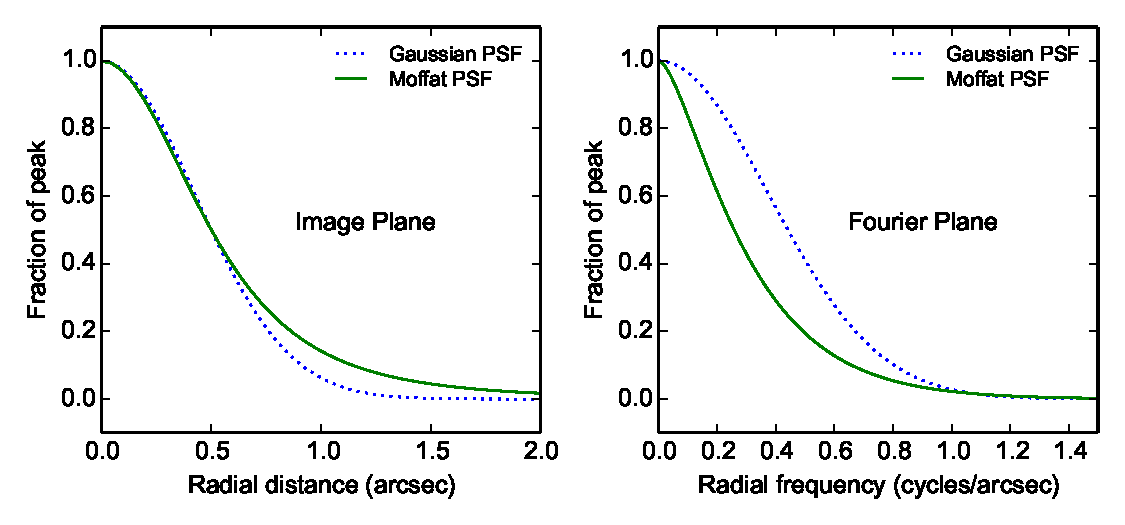
\includegraphics[width=4.5in]{psf_fft.pdf}
\caption{On the left, the radial cuts through a 2D Moffat PSF with
  FWHM=1.0 and $\beta=2.0$, and a Gaussian profile of the same FWHM
  for comparison.  On the right, the radial cuts through the 2D
  Fourier transforms of these PSFs.}
\label{moffat_psf_figure}
\end{center}
\end{minipage}
\end{center}
\end{figure}

The point-spread functions of astronomical observations are frequently
modeled as Moffat functions, following the work of
\cite{moffat1969}. This better models the PSF resulting from
atmospheric turbulence and telescope defects than a Gaussian. The peak
of a Moffat function is similar to a Gaussian, but further from the
peak it decreases more slowly than a Gaussian, by a degree that
depends on a parameter, $\beta$. When $\beta$ is unity, the Moffat
function is equivalent to a Lorenz function, which is a function that
falls much more slowly than a Gaussian. Increased values of $\beta$
result in ever closer approximations of a Gaussian function.

In the image plane, the radial profile of a two dimensional Moffat
function is defined as follows.

\begin{equation}
p(r) = \frac{\beta-1}{\pi\alpha^2}\frac{1}{\left(1+\frac{r^2}{\alpha^2}\right)^{\beta}}
\end{equation}

Where $\alpha^2$ is proportional to the full-width at half-maximum
(FWHM) of the Moffat function, as follows.

\begin{equation}
\alpha^2 = \frac{\mbox{\scriptsize FWHM}^2}{4(2^{\frac{1}{\beta}} - 1)}
\end{equation}

Unfortunately there is no analytic form for the Fourier transform of a
Moffat function, so to convolve an image with a Moffat PSF of a given
FWHM and $\beta$, it is necessary to first create an image of that
PSF, take the Fast Fourier Transform of both this and the image to be
convolved, multiply these in the Fourier plane, and then take an
inverse Fourier transform to obtain the convolved image. As described
in section~\ref{discrete_convolution}, care must be taken to ensure
that the image of the Moffat PSF is on a sufficiently fine grid as
that it is essentially Nyquist sampled.

The PSF of the MUSE image is adequately sampled by the MUSE pixel
grid, so a Moffat model of this can be sampled with the pixel spacing
of the MUSE image that is being characterized. This is not true for
the HST PSF, however. Although the HST PSF is adequately sampled by
the $0.03\arcsec$ pixel spacing of the original HST image, this pixel
spacing is about seven times smaller than the pixel spacing of MUSE
images, and a single pixel of a MUSE image is twice as wide as the
FWHM of the HST PSF. So the HST PSF must be sampled with pixels that
are at least seven times smaller than MUSE pixels. In practice a
factor of eight is used, for reasons that will become apparent.

If a two-dimensional image has $N_x \times N_y$ pixels, and a pixel
spacing of $d_x$ and $d_y$ arc-seconds along the X and Y axes, then
the FFT of this image has pixels in the Fourier plane that have
spacings of $\frac{1}{N_x d_x}$ and $\frac{1}{N_y d_y}$
cycles/arc-second along the X and Y frequency axes. To perform a
convolution by multiplying corresponding pixels of two discrete
Fourier transforms, the two Fourier transforms must have the same
pixel spacing in the Fourier plane. This is true if the products $N_x
d_x$ and $N_y d_y$ are the same for both images. So if the pixel
spacings of one of the images are decreased to $d_x/\rho$ and
$d_y/\rho$, then the array dimensions of that image must be increased
by the same amount, to $\rho N_x \times \rho N_y$. In practice, both
images should have array dimensions that are integer powers of two, to
optimize the speed of the FFT algorithm. If $N_x$ and $N_y$ are powers
of two, then the array dimensions of the more finely sampled image
will also be powers of two if the pixel size reduction factor is an
integer power of two. For this reason, a pixel-size reduction factor
of 8 is used to create the image of the Moffat model of the HST
PSF. In the Fourier plane, this results in a Fourier transform that
has 8 times as many pixels along each axis as the MUSE image to be
convolved. Only the inner $N_x \times N_y$ pixels of this FFT are used
to multiply the FFT of the MUSE image. Fortunately the large FFT of
the finely gridded HST PSF only has to be computed once, before the
fitting procedure begins.

\subsection{The Decimation Filter}

As described in section~\ref{sampling}, before resampling an image
onto a coarser grid, it should be smoothed by a decimation filter to
remove any flux at spatial frequencies above half the new sampling
rate. Resampling an HST image onto the pixel size of a MUSE image,
involves increasing the pixel size from $0.03\arcsec$ to $0.2\arcsec$,
which is a factor of almost seven.

\subsubsection{Filtering in the image domain}

To apply a decimation filter in the image domain one first needs to
obtain the inverse Fourier transform of the desired 2D filter curve,
sampled with the same pixel interval as the image. This is commonly
called a convolution kernel, and it is usually much smaller than the
image that is to be filtered. The image is convolved with this kernel
to filter it.

The width of the convolution kernel that is needed to implement a
decimation filter, can be estimated using the following equation,
which is derived from equation 5-49 of \cite{lyons2011}.

\begin{equation}
  N_w = \frac{\alpha f_s} {22 B_{tr}}
\end{equation}

This equation estimates the width of the convolution kernel of an FIR
filter with a given stop-band attenuation, $\alpha$ (dB), and a given
transition bandwidth between the pass-band and the stop-band. The
transition bandwidth, $B_{tr}$, is the frequency interval over which
the filter's response smoothly decreases from unity to the desired
stop-band attenuation. In the equation, $f_s$, is the sampling
frequency of the image before downsampling.

A reasonable stop-band attenuation is 60dB. When decimating an HST
image that has $0.03\arcsec$ pixels, $f_s$ is $1/0.03\arcsec$. The
sampling frequency of the resampled MUSE image is $1/0.2\arcsec$, and
the cutoff frequency of the low-pass filter should be about half this
frequency, $f_{cut}=1/0.4\arcsec$. The transition bandwidth of the
filter is a fraction of the cutoff frequency between 0 and 1. To
implement a filter that is essentially flat up to about half the
cutoff frequency, $B_{tr} =1/0.8\arcsec$. This yields $N_w = 72.7$
pixels. So to adequately filter an HST image before resampling it to
the MUSE pixel size, would require one to convolve it with a
convolution kernel of 73x73 pixels. That would be inefficient in the
image plane.

\subsubsection{Filtering in the Fourier domain}

Filtering the HST image in the Fourier domain is done by taking a Fast
Fourier Transform (FFT) of the HST image, multiplying this by a window
function that goes to zero at half the sampling rate of the MUSE pixel
grid, then performing an inverse FFT on the result, to obtain the
filtered HST image.

Before the performing the FFT, zero valued margins must be added
beyond the end pixels of the X and Y axes. The size of this margin
should be at least as large as the convolution kernel would have been
in the image plane, to avoid the wrap-around effects of circular
convolution.  Using the example given above for the requirements for
image-plane convolution, at least 73 pixels of zeros should be added
at the ends of the X and Y axes when decimating an HST image onto the
pixel grid of a MUSE image.

After padding the image with zeros to avoid circular convolution, the
margins should be widened if the image dimensions are not integer
powers of two. This is because FFTs can be extremely slow when applied
to images whose dimensions are not powers of two.

\subsubsection{The Decimation Filter Window Function}

\begin{figure}[htbp]
\begin{center}
\begin{minipage}[b]{5.5in}
\begin{center}
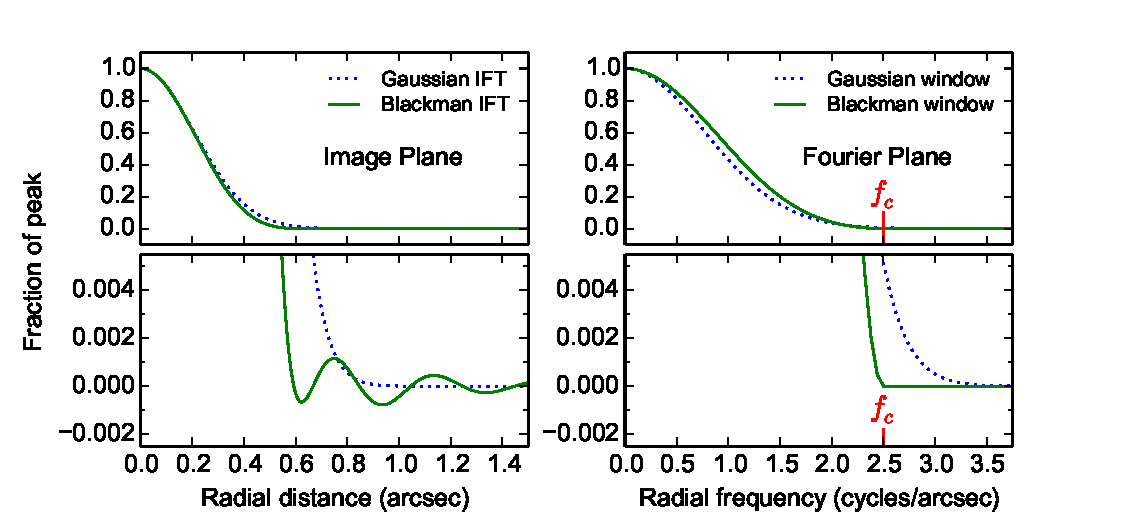
\includegraphics[width=5.0in]{blackman_ift.pdf}
\caption{The graphs on the right show radial cuts through circularly
  symmetric 2D Blackman and Gaussian window functions in the Fourier
  plane. The Blackman window has a cutoff frequency, $f_c$, of half
  the sampling rate of an HST image with $0.03\arcsec$ pixels. The
  graphs on the left show radial cuts through the 2D inverse Fourier
  transforms of these window functions, showing their effect on point
  sources. The width of the Gaussian window was chosen to make the
  FWHMs of the inverse Fourier transforms of both windows match in the
  image plane.}
\label{blackman_ift_figure}
\end{center}
\end{minipage}
\end{center}
\end{figure}

There are many commonly known window functions that could be used to
implement a decimation filter in the Fourier plane. However the one
that seems to be optimal from the point of view of avoiding the
appearance of ringing artifacts near bright point sources, saturated
regions and other abrupt changes in the image plane, seems to be the
Blackman window, which has a stop-band attenuation of 60dB. When used
to implement a decimation filter, it is defined as follows.

\begin{eqnarray}
w(k) &=& \left.0.42 + 0.5\cos\left(\frac{\pi f(k)}{f_c}\right) +
0.08\cos\left(\frac{2\pi f(k)}{f_c}\right)\,\right\vert_{|f(k)|\le f_c}\\
     &=& 0.0\ \vert_{|f(k)| > f_c}\nonumber
\end{eqnarray}

Where $f(k)$ is the spatial-frequency of pixel $k$ of the image, and
$f_c$ is the desired cutoff spatial-frequency. For a decimation
window, $f_c$ is half the sampling rate of the final image
(\textit{ie.} the MUSE image in our case).

To satisfy the sampling requirements for decimation, it would be
sufficient to apply the above window first along the X axis, then
separately along the Y axis. However this results in a PSF that is not
circularly symmetric. To make it circularly symmetric, $f_k$ should be
$\sqrt{f_x(k)^2 + f_y(k)^2}$, where $f_x(k)$ and $f_y(k)$ are the
spatial frequencies of pixel $k$ along the X and Y axes of the Fourier
transform, respectively.

The Blackman window completely cuts off frequency components above the
cutoff frequency. As can be seen in figure~\ref{blackman_ift_figure},
this results in low-level ringing in its point-source response in the
image plane, at a level of 1/1000 of the peak value.

A Gaussian window function could also be used for this
purpose. However a Gaussian window does not fall to zero at the cutoff
frequency. If the frequency coverage of the Fourier transform extends
significantly past the desired cutoff frequency, then the result will
be some low level aliasing. If the frequency coverage doesn't extend
far past the cutoff frequency, however, then the truncation of the
Gaussian window produces worse ringing in the image plane than the
Blackman window. In the plot, the FWHM of the Gaussian window in the
Fourier plane was set to:

\begin{equation}
  \mbox{guassian\_fwhm} = 0.72555 f_c
\end{equation}

Under the assumption that the Gaussian window in the Fourier plane
extends significantly beyond the cutoff frequency, this ensures that
the image-plane responses to the Blackman and Gaussian windows, have
matching FWHMs.

\section{Generating MUSE images with an HST filter-curve}

The HST cameras provide a selection of filters that can be used to
constrain the wavelength range of an observation. Of these, the F606W,
F775W, F814W and F850LP filters significantly overlap the wavelength
range of the MUSE spectrometer. HST observations taken with these
filters can be used with the technique described in this document, to
fit for the PSFs of MUSE images. For this to work well, the
corresponding MUSE images must have the same filter curve as the HST
observation. The MUSE IFS generates a cube of 3681 narrow-band images,
spaced in wavelength by $0.125\,\nm$, from $475\,\nm$ to
$935.125\,\nm$. To generate a MUSE image that has the filter curve of
an HST image, each narrow-band MUSE image is multiplied by the
integral of the HST filter-curve over its wavelength range, then the
scaled MUSE images are summed and divided by the integral of the
filter-curve over the range of the MUSE channels.

\begin{equation}
  f_m(x,y) = \frac{\sum_{i=1}^{N_{\lambda}}
  m_i(x,y)\cdot\int_{\lambda_i-\Delta\lambda/2}^{\lambda_i+\Delta\lambda/2} h_f(\lambda)\delta\lambda}{\int_{\lambda_1-\Delta\lambda/2}^{\lambda_{N_\lambda}+\Delta\lambda/2} h_f(\lambda)\delta\lambda}
\end{equation}

In the above equation, $m_i(x,y)$ represents the $i^{th}$ image of a
MUSE cube, $N_{\lambda}$ is the number of images in the cube,
$\lambda_i$ is the central wavelength of channel $i$ of the cube,
$\Delta\lambda$ is the width of a channel in the cube, and
$h_f(\lambda)$ is the interpolated value of the filter curve at
wavelength, $\lambda$. The final MUSE image is $f_m(x,y)$.

HST filter curves are not sampled at fixed wavelength intervals. To
interpolate each HST filter-curve, a cubic-spline is fit to it.

\appendix
\section{Convolution, Sampling and Fourier transforms}
\label{sampling_appendix}

The technique described in this document relies heavily on the
relationships between convolution, discrete sampling and Fourier
transforms, so this appendix has been added to clarify them.

\subsection{The Convolution theorem}

The convolution theorem is fundamental to understanding the
relationships between sampling, convolution and Fourier
transforms. The convolution theorem simply states that convolution and
multiplication are Fourier transform pairs. Specifically, if $f(t)$
and $g(t)$ are continuous functions of time, and $F(\nu)$ and $G(\nu)$
are their continuous Fourier transforms versus frequency, then:

\begin{eqnarray}
f(t)\ast g(t) &\ftarrow& F(\nu)\cdot G(\nu) \\
f(t)\cdot g(t) &\ftarrow& F(\nu)\ast G(\nu)
\end{eqnarray}

Where $\ast$ denotes convolution, and $\cdot$ denotes multiplication.

\subsection{Commutative and Associative properties of convolution}

Since multiplication is commutative, associative and distributive, it
follows that convolution has these properties too, because the Fourier
transform of a convolution is a multiplication and the Fourier
transform of a sum of two terms is the sum of the Fourier transforms
of those terms. For example, the right hand sides of the following two
equations have the same values, because the operands of a
multiplication can be swapped without changing the result, so
$f(t)\ast g(t) = g(t) \ast f(t)$.

\begin{eqnarray}
f(t)\ast g(t) &\ftarrow& F(\nu) \cdot G(\nu) \\
g(t)\ast g(t) &\ftarrow& G(\nu) \cdot F(\nu)
\end{eqnarray}

Similarly in the following equation, the associative property of
multiplication means that the terms of the right hand side of the
equation can be reordered without changing its value. Since the
ordering on the right hand side reflects the order of the convolution
operands on the left hand side, this indicates that the order of the
convolutions is equally unconstrained, so convolution is also
associative.

\begin{eqnarray}
\{f(t) \ast g(t)\} \ast h(t) \ftarrow \ft\left\{f(t) \ast g(t)\right\}
\cdot H(\nu) = F(\nu) \cdot G(\nu) \cdot H(\nu)
\end{eqnarray}

Finally, it is clear that the right hand sides of
equations~\ref{assoc1_eqn} and \ref{assoc2_eqn}, have the same values,
and this demonstrates that convolution is distributive.

\begin{eqnarray}
f(t) \ast [g(t) + h(t)] &\ftarrow& F(\nu)\cdot \ft\{g(t)+h(t)\}
\nonumber \\
\label{assoc1_eqn}
                               &=& F(\nu)\cdot [ G(\nu) + H(\nu) ]\\
\label{assoc2_eqn}
f(t) \ast g(t) + f(t) \ast h(t) &\ftarrow& F(\nu)\cdot G(\nu) +
F(\nu)\cdot H(\nu)
\end{eqnarray}

\subsection{Sampling of continuous functions}
\label{sampling}
A continuous function, $f(t)$, that is sampled at regular intervals,
$\tau$, can be written as the product, $\sha_{\tau}(t) \cdot f(t)$,
where $\sha_{\tau}(t)$ is a Dirac comb of period $\tau$.  According to
the convolution theorem, the Fourier transform of this product is a
convolution of the Fourier transform of $\sha_{\tau}(t)$ with the
Fourier transform of $f(t)$.  The Fourier transform of
$\sha_{\tau}(t)$ is another Dirac comb of period $1/\tau$, so the
result can be written as follows.

\begin{equation}
  \sha_{\tau}(t) \cdot f(t) \ftarrow \sha_{\frac{1}{\tau}}(\nu) \ast F(\nu)
\end{equation}

The convolution of $F(\nu)$ with $\sha_{\frac{1}{\tau}}(\nu)$,
generates a periodic sum of copies of $F(\nu)$, shifted by successive
intervals of $1/\tau$ Hz. If $f(t)$ has been low-pass filtered to
remove frequency components above $\frac{1}{2\tau}$, then each period
of this sum is identical to a shifted copy of $F(\nu)$. However this
is not true if $f(t)$ contains any frequencies above
$\frac{1}{2\tau}$, because then $F(\nu)$ is so wide that neigboring
copies of $F(\nu)$ overlap in the sum. The overlap is known as
aliasing, which converts high frequency components of $f(t)$ into
undesirable low frequency artifacts in the sampled signal. To avoid
aliasing, one can either sample at a frequency that is greater than
twice the highest frequency in $f(t)$, or low-pass filter $f(t)$ to
remove frequencies above half the desired sampling rate.

The filter that is used to remove high frequencies is commonly known
as a decimation filter or anti-aliasing filter. This filter needs to
be applied before sampling a continuous analog signal, and also when
data that have already been sampled, are re-sampled onto a coarser
grid. Failure to apply a decimation filter results in low-frequency
artifacts such as ringing next to steps in the image plane, increased
noise due to high frequency noise being folded to lower frequencies,
and the elimination of small features that happen to lie between the
sampling points of the coarser grid.

When the pixel size of an array is to be increased by an integer
factor, $N$, it is tempting to calculate the new pixel values as sums
of successive sequences of $N$ pixels.  However each of these sums
acts like a boxcar decimation filter.  In the Fourier plane this is
equivalent to multiplying the Fourier transform of the data by the
main lobe of a sync function. The first zero of this sync function is
at half the sampling frequency of the new pixel size, so at that
frequency it meets the Nyquist sampling requirements. However the sync
function has significant sidelobes at higher frequencies, so any noise
or sharp edges at those frequencies are still aliased to lower spatial
frequencies in the re-sampled data.

Rather than summing neighboring pixels with equal weights, it is
better to apply a well designed low-pass filter to the data, then
sub-sample or interpolate the smoothed data. When down-sampling an
image, the decimation filter can be applied in the spatial domain, by
convolving the image with a smoothing kernel. Alternatively it can be
done by taking the Fourier transform of the data, multiplying this by
a window function that falls smoothly to zero at half the sampling
rate, then performing an inverse Fourier transform to recover the
smoothed data. The image-plane approach is faster for small decimation
factors. However its processing time increases as the square of the
decimation factor, so Fourier plane filtering is faster for large
decimation factors.

\subsection{The Convolution of two Discrete functions}
\label{discrete_convolution}

The convolution theorem refers to the convolution of continuous
functions. Some care must be taken when using discrete Fourier
transforms to perform convolution.  To convolve two continuous
functions whose Fourier transforms are not known, the obvious approach
is to grid these functions in the image plane, use the FFT algorithm
to obtain their discrete Fourier transforms, multiply the discrete
Fourier transforms together, and then perform an inverse FFT to obtain
a discrete version of the convolved function. The assumption in this
procedure is that the following equation is valid.

\begin{equation}
\label{discrete_conv_eqn}
 [\sha_{\tau}(t) \cdot f(t)] \ast [\sha_{\tau}(t) \cdot g(t)] \equiv
 \sha_{\tau}(t) \cdot [f(t)\ast g(t)]
\end{equation}

If this is true, then the Fourier transforms of the two sides of the
above equation should also be equivalent, as follows.

\begin{equation}
\label{ft_discrete_conv_eqn}
[\sha_{\frac{1}{\tau}}(\nu)\ast F(\nu)] \cdot [\sha_{\frac{1}{\tau}}(\nu)\ast
   G(\nu)] \equiv \sha_{\frac{1}{\tau}}(\nu)\ast [F(\nu) \cdot
  G(\nu)]
\end{equation}

These Fourier transforms are periodic with a period of
$\frac{1}{\tau}$, so if both sides are equivalent within the frequency
range, $-\frac{1}{2\tau}\leq\nu\leq\frac{1}{2\tau}$, then they are
also equivalent at all frequencies. If $f(t)$ and $g(t)$ have both
been band-limited to suppress frequencies above $\frac{1}{2\tau}$,
then within this frequency range of the Fourier transform,
$\sha_{\frac{1}{\tau}}(\nu)\ast F(\nu) = F(\nu)$ and
$\sha_{\frac{1}{\tau}}(\nu)\ast G(\nu) = G(\nu)$. Thus the left hand
side of equation~\ref{ft_discrete_conv_eqn} is identical to $F(\nu)\cdot
G(\nu)$ over one period of the Fourier transform. Similarly, if $f(t)$
and $g(t)$ are bandlimited, then so is $f(t)\ast g(t)$, so the left
hand side of equation~\ref{ft_discrete_conv_eqn} is also identical tor
$F(\nu)\cdot G(\nu)$ over one period of the Fourier transform. Thus
equations~\ref{discrete_conv_eqn} and \ref{ft_discrete_conv_eqn} are valid if
both $f(t)$ and $g(t)$ are appropriately band-limited.

The above equations are not valid, however, if either of $f(t)$ or
$g(t)$ is undersampled, and the aliased frequencies of that function
overlap with non-zero parts of the spectrum of the other function. So
when convolving an image with an analytic function that is narrow in
the image plane, it is essential that the analytic function be sampled
adequately in the image plane to avoid aliasing. For example, when
convolving a low resolution image with the PSF of a much higher
resolution image, it is likely that the PSF is undersampled by the
sampling interval of the lower resolution image, so the PSF must be
sampled on a finer grid than the lower resolution image before it is
Fourier transformed.

When an image is to be convolved with a 2D function that needs to be
sampled onto a finer grid than the image, it is beneficial to sample
the function onto a grid that covers the same area as the image, but
that divides this area into a larger number of pixels. In the Fourier
plane, the spatial-frequency sampling interval is set by the overall
width and height of the image that is Fourier transformed, not by the
pixel size in the image plane, so by doing this, the innermost pixels
of the FFT of the more finely sampled function have the same spatial
frequencies as the FFT of the image, and these can then be multiplied
with those of the image to perform the convolution.

\subsection{Convolution of Discrete and Continuous Functions}

When an image is to be convolved with a function whose continuous
Fourier transform is known, there is no need to perform a discrete
Fourier transform of the function, so there is no need to worry about
aliasing of this function. In this case one takes the FFT of the
image, multiplies this by the analytical Fourier transform of the
function to be convolved, then performs an inverse FFT to obtain the
gridded version of the convolution.

\begin{equation}
 [\sha_{\tau}(t) \cdot f(t)] \ast g(t) \ftarrow
 [\sha_{\frac{1}{\tau}}(\nu)\ast F(\nu)] \cdot G(\nu)
\end{equation}

The result of the multiplication on the right hand side of the above
equation is clearly a function that is sampled at frequency intervals
of $\frac{1}{\tau}$, which means that the result of the convolution,
on left hand side of the equation, is still sampled on the original
image grid. We also know that if $f(t)$ is a band-limited function,
with no frequency components above $\nu>\frac{1}{2\tau}$, then
$[\sha_{\frac{1}{\tau}}(\nu)\ast F(\nu)]$ is identical to $F(\nu)$
within one period of the periodic Fourier transform of the right hand
side, so the sampled left hand side of the equation, in this case must
be the same as $\sha_{\tau}(t) \cdot [f(t)\ast g(t)]$. So the
conclusion is that:

\begin{equation}
\label{discrete_cont_conv_eqn}
 [\sha_{\tau}(t) \cdot f(t)] \ast g(t) \equiv \sha_{\tau}(t) \cdot [f(t)\ast g(t)]
\end{equation}

\bibliographystyle{authordate1}
\bibliography{muse_psf_fitting.bib}

\end{document}
